\documentclass{article}
\usepackage[a4paper, margin=2cm]{geometry}
\usepackage{amsmath, commath, physics}
\newcommand{\iu}{\mathrm{i}\mkern1mu}

% Colors
\usepackage{xcolor}
\definecolor{xred}{HTML}{BD4242}
\definecolor{xblue}{HTML}{4268BD}
\definecolor{xgreen}{HTML}{52B256}
\definecolor{xpurple}{HTML}{7F52B2}
\definecolor{xorange}{HTML}{FD9337}
\definecolor{xdotted}{HTML}{999999}
\definecolor{xgray}{HTML}{777777}
\definecolor{xcyan}{HTML}{80F5DC}
\definecolor{xpink}{HTML}{F690EA}
\definecolor{xgrayblue}{HTML}{49B095}
\definecolor{xgraycyan}{HTML}{5AA1B9}

% Graphics and figures
\usepackage{tikz, pgfplots}
\usetikzlibrary{arrows}
\tikzset{
	vector/.style={-stealth, ultra thick, cap=round},
    coordline/.style={very thick, dotted, black!75},
}
\pgfplotsset{
	compat=1.16,
	%% Styles %%
	xyplane/.style = {
			axis equal,
			axis x line=middle,
			axis y line=middle,
			xlabel=$x$,
			ylabel=$y$,
			every axis x label/.style={at={(ticklabel* cs:1.0)}, anchor=west},
			every axis y label/.style={at={(ticklabel* cs:1.0)}, anchor=south},
			axis line style={stealth-stealth, black, line width=0.5pt},
			% label style={font=\large},
			% tick label style={font=\large},
			samples=250,
			xmin=-5, xmax=5,
			ymin=-5, ymax=5,
			grid=both,
			major grid style={black!5},
			minor grid style={black!2},
			minor tick num = 5,
			xticklabels={,},
			yticklabels={,},
			restrict y to domain=-10:10
		},
    complexplane/.style = {
        xyplane,
        xlabel=$\Re$,
        ylabel=$\Im$,
    },
	xynogrid/.style={
			xyplane,
			major grid style={opacity=0},
			minor grid style={opacity=0},
		},
	xynoaxes/.style={
			xyplane,
			axis line style={draw=none},
			xlabel={}, ylabel={},
			extra x tick labels={,},
			extra y tick labels={,},
			tick style={draw=none},
		},
	xyempty/.style={
			xyplane,
			axis line style={draw=none},
			tick style={draw=none},
			xlabel={},
			ylabel={},
			major grid style={draw=black!0},
		},
}


\setlength{\parindent}{0cm}

\title{Introduction to Complex Numbers and Their Uses}
\author{Peleg Bar Sapir}

\begin{document}
\maketitle

\section{Real, "Imaginary" and Complex Numbers}
\begin{figure}
	\begin{center}
		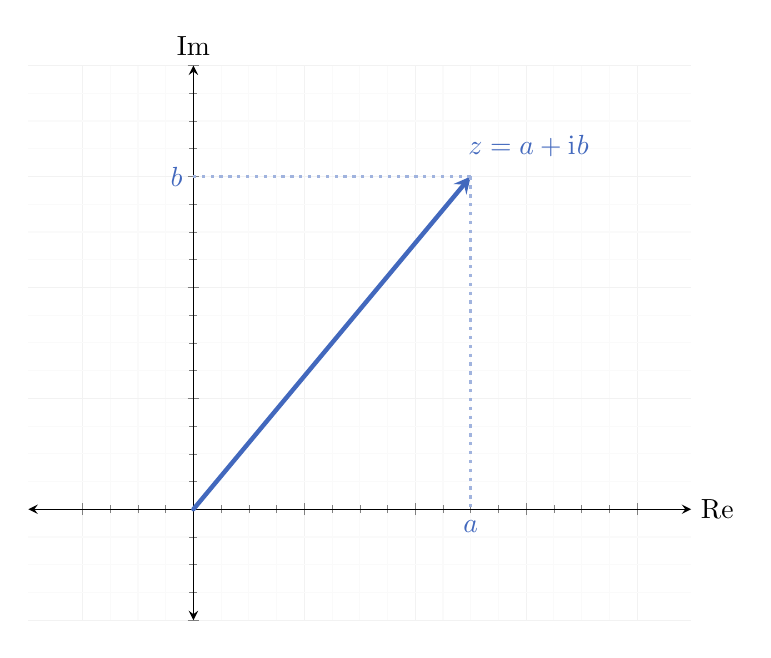
\begin{tikzpicture}[scale=1]
			\def\zcol{xblue}
			\begin{axis}[
					width=10cm,
					complexplane,
					xmin=-1, xmax=4,
					ymin=-1, ymax=4,
					xtick={-1,...,4},
					ytick={-1,...,4},
					minor tick num=3,
				]
				\pgfmathsetmacro{\a}{2.5}
				\pgfmathsetmacro{\b}{3.0}
				\draw[vector, \zcol] (0,0) -- (\a,\b) node [anchor=west, pos=1.05, xshift=-10pt, yshift=5pt] (z) {$z=a+\iu b$};
				\draw[coordline, \zcol!50] (\a,\b) -- (\a,0) node[below, \zcol] {$a$};
				\draw[coordline, \zcol!50] (\a,\b) -- (0,\b) node[left, \zcol] {$b$};
			\end{axis}
		\end{tikzpicture}
	\end{center}
	\caption{This is a test figure.}
	\label{fig:testfig}
\end{figure}

\section{Algenraic Properties}
\section{Polar (Geomteric) Representation}
\section{Exponential Representation}
\section{Complex Functions}
\section{Higher-dimension Forms}
\section{Uses}

% section  (end)

\end{document}
